
\begin{figure*}[t]
  \centering
  % \includegraphics[width=\textwidth]{icml2026/figures/execution-trace.pdf}
  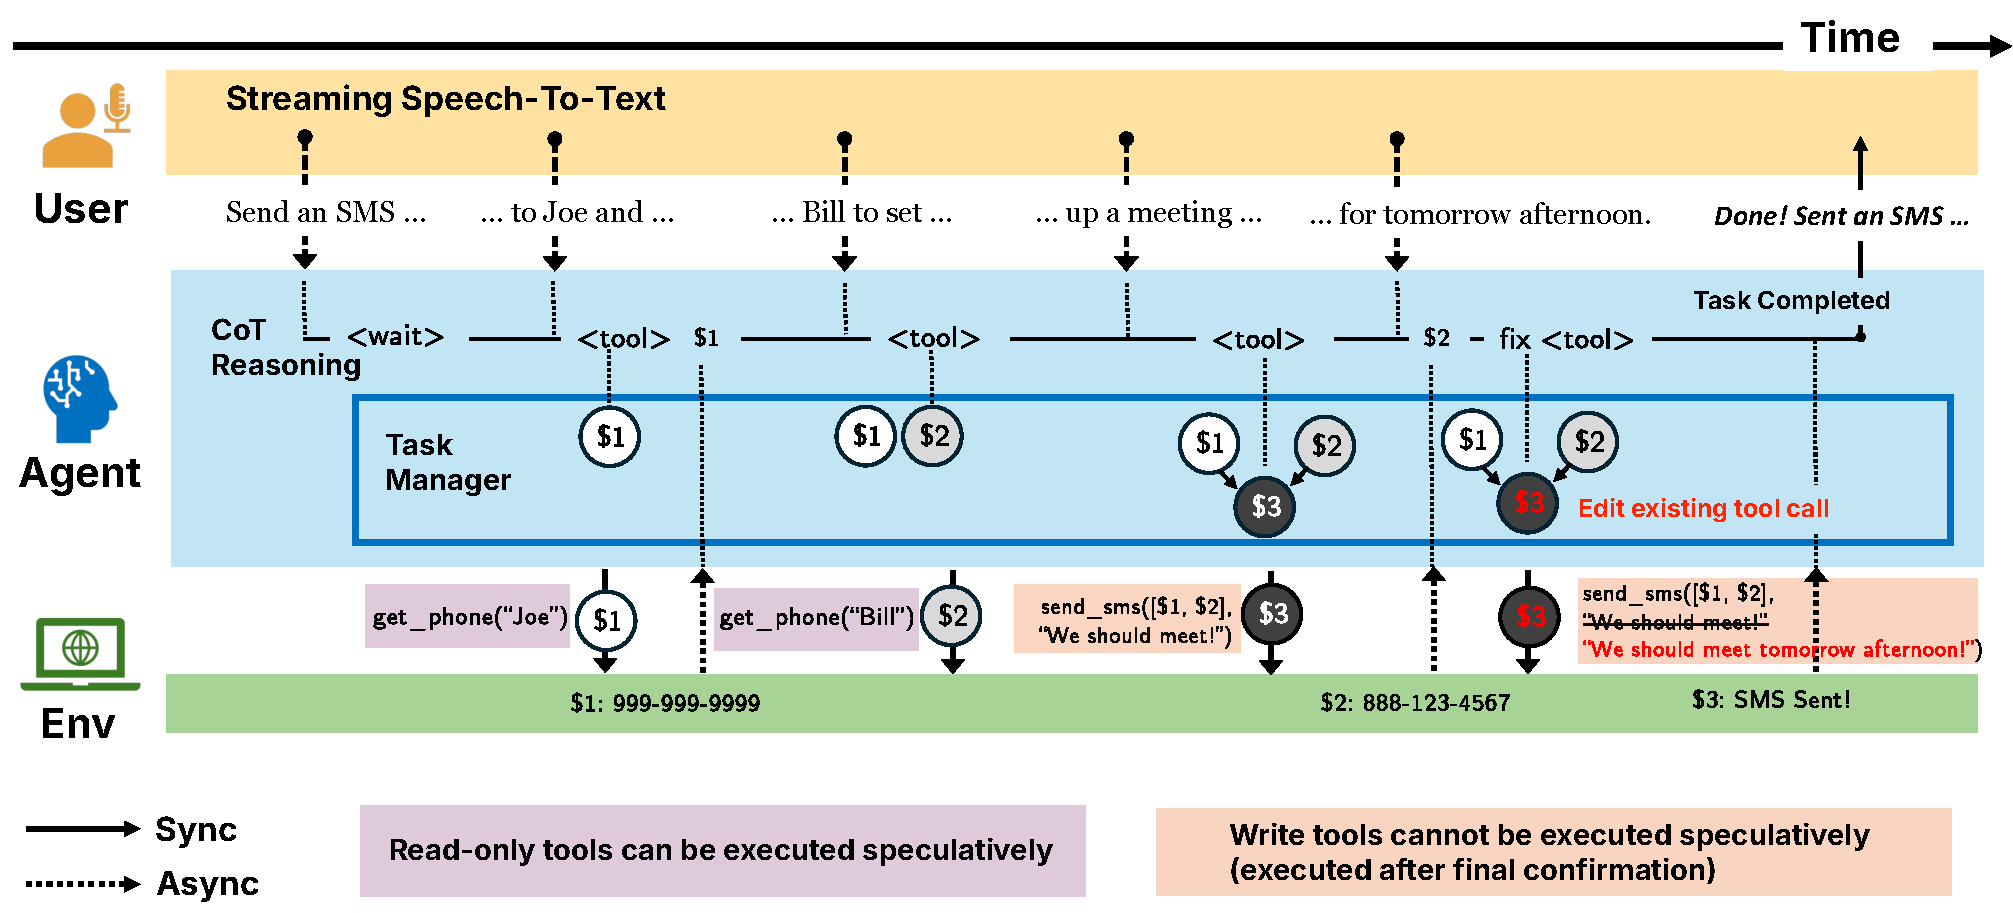
\includegraphics[width=\textwidth]{figures/figure2.pdf}
  \caption{ 
  \textbf{Example Execution Trajectory.} An example trajectory showing agent execution unrolled over time, demonstrating how the agent reasons and acts continuously while waiting on additional user information as well as tool execution. 
  The diagram also highlights how tool calls can be generated based on partial user inputs, and how tool calls can later be modified after receiving more information to ensure the updated tool calls are aligned with the user query.
  Note that only read-only tools can be executed before receiving a final confirmation signal to avoid irreversibly modifying system state.
  }
  % \vspace{-3mm}
  \label{fig:execution-trace}
\end{figure*}


\section{Related Work}

Here, we provide a brief summary of related work on efficient language and voice agents as well as related system infrastructure projects.
A more detailed description of related work and comparison with our method is provided in Appendix \ref{sec:appendix_related_work}.

\subsection{Efficient LLM Agents}

Several prior works have explored how to execute agentic workflows more efficiently, including parallelizing tool calls where possible \citep{kim2024llm} and performing work while waiting on asynchronous tool execution responses \citep{gim2024asynchronous}.
Another prior work used separate thinker and talker threads so that one thread could talk to the user while the other thread performed a background reasoning process \citep{yakushev2025asynchronous}.
An additional concurrent work trained an ``Interaction Model" to respond in real-time to the user, while delegating complex reasoning to a background thread \cite{thinkingmachines2026interactionmodels}.
There has also been work on designing proactive and interactive LLM agents, including Pepper \citep{rllm2025pepper}, which proposed an event-driven architecture for proactive LLM assistants.
Compared with prior work, our work builds on the asynchronous tool calling method from \citep{gim2024asynchronous} and generalizes this to handle both asynchronous user updates as well as asynchronous responses from the environment.
Our work also builds on the decoupled planning/execution from LLMCompiler \citep{kim2024llm}, which allows for tool calls to be executed in parallel as soon as their operands are ready.
We extend this to allow for issuing tool calls iteratively as we obtain sufficient information, and also propose \textit{Speculative Tool Calling} (Sec. \ref{sec:spec-tool-calling}) to hold up sensitive tool calls until they are confirmed and to allow for modifying/removing tool calls that have been issued but not yet finished execution.

\subsection{Efficient Voice Agents}

There has also been prior works that have explored methods to accelerate voice agents by exploiting the streaming nature of speech.
StreamRAG \citep{arora2025stream} proposes launching RAG calls partway through receiving the streaming user input, thereby reducing response latency.
SHANKS \citep{chiang2025shanks} processes the streaming input speech in fixed chunks and interleaves unspoken reasoning (as well as tool calls) between chunks while waiting for further information from the user, whereas STITCH \citep{chiang2025stitch} interleaves text-to-speech with unspoken reasoning.
Our approach builds on \citep{chiang2025shanks} by pursuing a similar approach where we interleave reasoning and acting with streaming input speech. 
The key differences with our method are 1) we support asynchronous tool calling as well as asynchronous user inputs, 2) we propose \textit{Speculative Tool Calling} (Sec. \ref{sec:spec-tool-calling}) to handle sensitive tool calls and cases where the tool call is issued incorrectly with partial information. 

\subsection{System Support for Streaming Inference}

There has also been recent work on system-level optimizations to enable real-time interactive agentic systems.
The OpenAI Realtime API \citep{openai_realtime_api} and Gemini Live API \citep{GoogleLiveAPI2025} both provide websocket-based interfaces that support streaming inputs (for reducing TTFT due to prefilling latency) and outputs (producing partial responses that can start being returned to the user before the full output is available).
Additionally, open-source serving frameworks like vLLM have recently added support for efficient streaming input processing \citep{vllm2026streaming}.
There has also been efforts to design infrastructure for efficient streaming processing at the edge \citep{jeffries2024moonshine}.
